\chapter{Lightweight Real-Time Feature Monitoring} \label{chap:my-work} \minitoc

\section{Approach A: Usage of outlier detection methods}
The first approach considered relied on outlier detection methods such as the ones presented in Section \ref{sec:outliers} and classified by the taxonomy in Figure \ref{fig:outlier-taxonomy}. This straightforward approach works with either subsequence or point outlier detection methods to analyze the streaming sliding window and produce data pattern shift alerts.

\subsection*{How}

Using point outlier detection methods, the main idea would be to keep track of the rate of point outliers detected. For instance, keep track of how many outliers were alerted in the past hour. The decision to alert for a data pattern shift of the system would be made when comparing this rate of point outliers detected in the past hour with a user-defined threshold $\alpha$. On the other hand, using subsequence outlier detection methods would allow us to report the whole sliding window as an outlier. 


\subsection*{Challenges}
The analyzed outlier detection algorithms in Section \ref{sec:outliers} were deemed unfit for our use-case due to one or more of the following: \textit{(a)} high memory consumption, \textit{(b)} high time complexity, \textit{(c)} "memory loss" and \textit{(d)} obfuscated insights.

In our lightweight real-time solution we need constant time complexity to process events one by one in real-time. Additionally, because our system is not mission-critical, we want a solution as lightweight as possible, which means something that grows linearly with window size is not a good fit. Therefore, most of the outlier detection methods presented become unfit for our use due to high memory consumption and time complexity. Some of the methods shown also suffer from what we call \textit{"memory loss"}: they lose track of the reference window or normality period. In other words, the algorithms are online learners, meaning they adapt to the underlying statistics of the data stream. While in some scenarios this is a much-needed feature, in our use-case it is not. How clear the alerts and insights retrieved from the methods are is also an important property. Some outlier detection methods used Machine Learning (ML) techniques to produce alerts, which makes it harder to explain to a system administrator why an alert was raised and what changed.

\subsection*{Conclusion}
We concluded that employing outlier detection methods was not the best course of action and put aside this approach.

\section{Approach B: Thresholding aggregation values}
This second approach focus on building an aggregation snapshot of the reference period to compare with streaming aggregation values and alert if the difference between both surpasses a threshold $\alpha$.

\subsection*{How}

In this approach we compute sliding window aggregations and compare the aggregations’ current state versus an initial reference, reporting a shift when the difference is substantial. For instance, consider the case where we monitor one single feature or variable \textit{x}. Assume we define the set of aggregations to compute the mean of \textit{x} and its standard deviation. Also assume we save the reference window and maintain a sliding window and the average and standard deviation aggregations for \textit{x} efficiently. As seen in Figure \ref{fig:approach2-initial-state}, the initial mean and standard deviation values for \textit{x} presented in the reference window are of 5 and 1, respectively. Later on, in \textit{Window 1}, we see the same values for the mean and standard deviation, of 5 and 1, respectively. This represents a \textit{normal} case where no alert is produced.

\begin{figure}[!htb]
    \begin{center}
      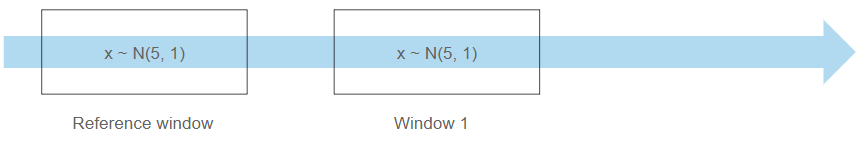
\includegraphics[scale=0.65]{figures/approach2-normality.png}
      \caption[]{Normal state for feature \textit{x} in window 1}
      \label{fig:approach2-initial-state}
    \end{center}
\end{figure}


In Figure \ref{fig:approach2-alert-state}, after further sliding steps of our sliding window, we obtain \textit{Window 2}. In \textit{Window 2}, the mean and standard deviation aggregation values change from 5 and 1 to 12 and 6, respectively. In this case, we would measure the difference between the sliding window aggregations and the reference window ones and if above a certain threshold raise an alert. For example, if we used a threshold of $\alpha$ = 6, we would raise an alert, as at least one sliding aggregation, in this case the mean, would differ of at least $\alpha$ when compared to the reference value.

\begin{figure}[!htb]
    \begin{center}
      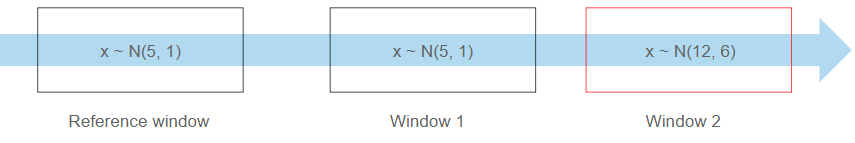
\includegraphics[scale=0.65]{figures/approach2-alert.png}
      \caption[]{Alert state for feature \textit{x} in window 2}
      \label{fig:approach2-alert-state}
    \end{center}
\end{figure}

\subsection*{Challenges}
The first issue with this approach is that generic sliding window aggregation algorithms grow linearly in space regarding window size, such as Recalculate-From-Scratch and Subtract-On-Evict presented in Section \ref{sec:back-swag-algs}, Two-Stacks has seen in Section \ref{sec:2stacks} and DABA in Section \ref{sec:daba}. Another challenge when using this approach is defining the set of aggregations to compute at feature/variable level that represent the system state well enough for comparison of reference and streaming periods and change detection. Yet another challenge would be to define the maximum deviation threshold $\alpha$  between the reference aggregation state and the streaming aggregation state to produce alerts.


Exponential Moving Averages (Section \ref{sec:emas}), Probabilistic Data Structures (Section \ref{sec:pds}) and their sliding window implementations (Section \ref{sec:sliding-pds}) can be used to solve the first issue and reduce the linear memory complexity of the system relative to sliding window size. 

However, there is no trivial solution for the second and third challenges. Defining the maximum allowed threshold between reference and sliding window aggregations does not have a straightforward solution. Furthermore, defining the set of aggregations to use is also a big challenge. To illustrate, consider both time-series show in Figure \ref{fig:approach2-timeseries}.
 
\begin{figure}[!htb]
    \begin{center}
      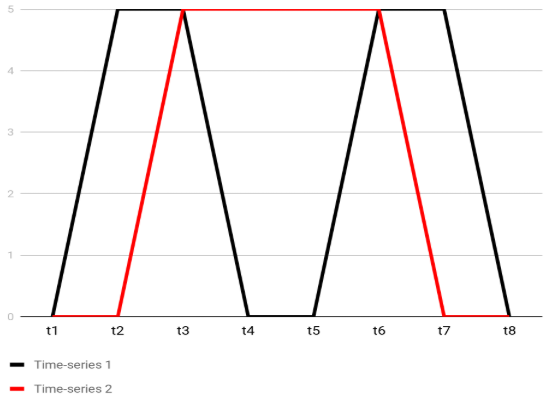
\includegraphics[scale=0.7]{figures/approach2-timeseries.png}
      \caption[]{Two different time-series with same max, min, mean and standard deviation}
      \label{fig:approach2-timeseries}
    \end{center}
\end{figure}


Both time-series 1 and 2 have the same maximum, minimum, mean and standard deviation values for the time-based window between \textit{t\textsubscript{1}} and \textit{t\textsubscript{8}}. Hence, if our set of aggregations chosen were the maximum, minimum, mean and standard deviation, we would not differentiate between these two clearly different time-series.

\subsection*{Conclusion}
This approach requires efficient sliding window aggregation state maintenance, which can be done using sliding window probabilistic data structures and/or exponential moving averages. However, defining the set of aggregations to use and the deviation threshold itself ultimately led us to discard this approach.


\section{Proposed method: Numerical Feature Monitoring}

Our goal is to detect data pattern shifts in an online fashion. Such shifts will be measured between a reference or normality period versus the observed reality during the streaming phase. Note that we need not to directly compare the entire window contents of the reference period with the contents of the sliding window. Doing this would require storing all window contents hence making our memory consumption grow linearly with sliding window and/or reference period size. We want some sort of aggregation over the reference period that can be maintained efficiently throughout run-time and can be used to distinguish both periods of time and alert for changes. In short, we want a reference aggregation snapshot to compare with a streaming aggregation that must be updated in real-time and constant in memory usage.

To that end, we devise a two-phased method. The first phase relies on a batch analysis that builds our aggregated reference snapshot to be later on compared with the sliding one. The second phase focus on efficiently updating the sliding window aggregation snapshot and occasionally perform a similarity test between the static reference aggregation and the sliding one, alerting for changes if need be. The proposed method currently works only for numerical features, that is, only for event fields or variables that are of numeric type, but can be extended to other types as well, as we will discuss.

\subsection{Stream monitoring goals}
Before diving into the batch and streaming algorithms we must further define our goal. In this Section we pose the question: \textit{"what is our goal during the streaming or monitoring phase?"} and answer it.

A data stream is an infinite stream of events. Each event is timestamped and contains multiple fields. In the context of this Thesis, each of the event's fields are also named features or time-dependent variables. You can think of them as columns in a traditional relational database table. Given this context, our goal is to produce alerts of the following form:

\[\textit{timestamp: [(x1, 0.23), (x2, 0.51), (x3, 0.55)}]\]

The format used allows us to know the \textit{timestamp} for the given alert, which features diverge (in this case \textit{x1, x2, x3}) and a value representative of how much each feature diverges (for instance, a float value between 0 and 1 that works as a confidence value). 

An alert should be raised if a feature distribution changes considerably. This immediately poses challenges such as \textit{(a)} finding a suitable aggregation that encodes each feature's distribution and allows for a change detection test and \textit{(b)} defining a deviation threshold $\alpha$.

\subsection*{Approximated Histogram Aggregation} \label{sec:ema-hist}

We chose to encode a feature distribution as a histogram. A histogram is an aggregation that represents the distribution of numerical features. However, we must recall that we need to update this histogram in constant time in a sliding window fashion, implying eviction of old elements and insertion of new ones must be done with \textit{O(1)} time complexity.

An exact histogram aggregation must keep the entire sliding window in memory...

\textcolor{red}{TODO: review this section after EMAs is written}

\subsection*{Defining the deviation threshold}

Assume we use a distance function that takes two histograms --- our reference aggregation histogram and our sliding window aggregation histogram --- and outputs a distance value. How do we threshold this value? For instance, consider the following left and right skewed distance distributions represented by Figures \ref{fig:skewed-left-distro} and \ref{fig:skewed-right-distro}, respectively. Note that these histograms do not represent the reference and/or sliding window aggregation histogram. Here we make the assumption we have an histogram that encodes the distribution of distance values measured between the reference aggregation and the sliding window aggregation.

\begin{figure}[!htb]
    \begin{center}
      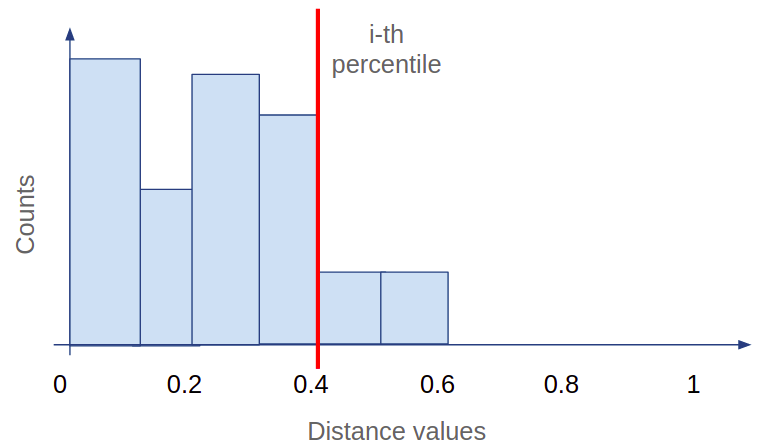
\includegraphics[scale=0.4]{figures/skewed-left-distro.png}
      \caption[]{Left skewed distribution of distance values}
      \label{fig:skewed-left-distro}
    \end{center}
\end{figure}

\begin{figure}[!htb]
    \begin{center}
      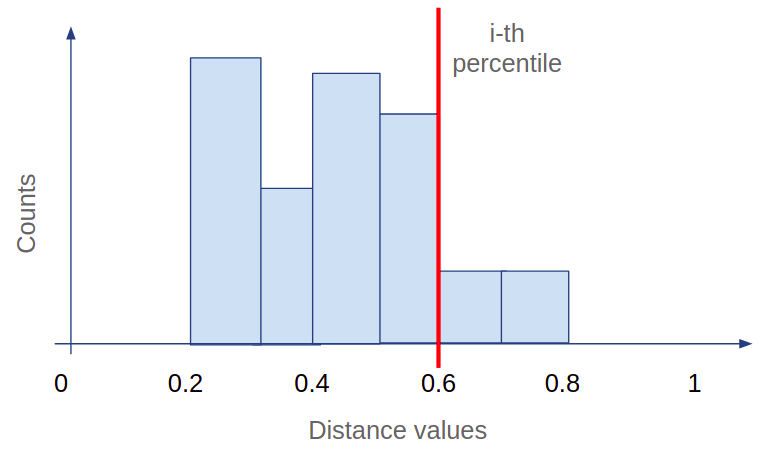
\includegraphics[scale=0.4]{figures/skewed-right-distro.png}
      \caption[]{Right skewed distribution of distance values}
      \label{fig:skewed-right-distro}
    \end{center}
\end{figure}

Let's assume Figure \ref{fig:skewed-left-distro} 's histogram encodes the distribution of expected distance values for a feature \textit{x1} and Figure \ref{fig:skewed-right-distro} does the same but for a feature \textit{x2}. Setting a user-defined threshold of \textit{$\alpha$=0.6} for both features would yield very different results. For feature \textit{x1} we would be reporting distance values above the 100th-percentile which would not be the case for feature \textit{x2}. Instead what we aim to do is know this distribution so that we can define our threshold as a percentile and not an hard-coded distance constant. For instance, in this case we would define the threshold to be the \textit{i}-th percentile, which would correspond to a threshold value of 0.4 for feature \textit{x1} and 0.6 for feature \textit{x2}.

Hard-coding a threshold value to be used for all features is cumbersome, impractical and error prone. The distance threshold must be computed based on the distribution of distances. How do we get to know the distribution of such distances? That is one of the goals for the batch phase.

\subsection{Batch analysis phase}
The goal of the batch phase will be to build our reference snapshot and get to know the distribution of "distances" between the reference snapshot and the sliding window one. In other words, we obtain a reference aggregation histogram that we later on use to measure its distance to the sliding window aggregation histogram, producing a distance value. We compare the measured distance with its distribution to find out how probable it is and alert in a very unlikely scenario. We do this for each feature.

\subsubsection*{Building the reference histogram for each feature}

First, for each feature, we compute the reference histogram from the reference period dataset. This is an exact histogram aggregation. When building it we ensure the histogram has equal counts (or equal height) for all bins which often results in different sized bins. We make no assumption on the dataset distributions and hence use equal height histograms because they adjust better to wildly varying ones. Equal height means we have more bins covering very dense regions (regions with many data points) and less bins in lower density regions. 

\begin{figure}[!htb]
    \begin{center}
      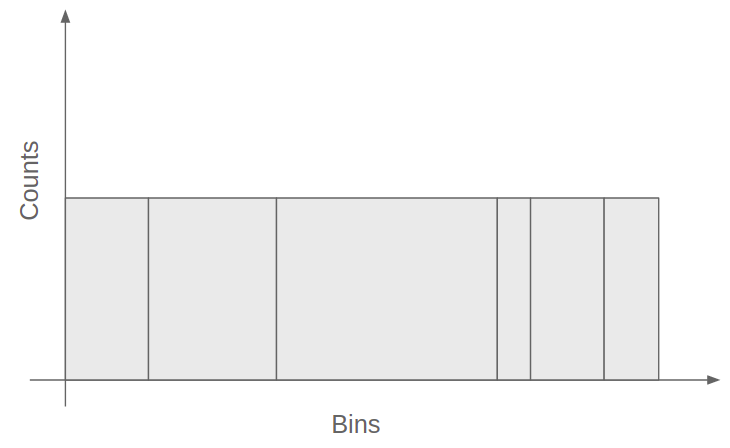
\includegraphics[scale=0.4]{figures/ref-hist.png}
      \caption[]{Reference equal-height histogram}
      \label{fig:ref-hist}
    \end{center}
\end{figure}


\subsubsection*{Finding the distribution of distances for each feature}
Secondly, we aim to build the histogram that encodes the distribution of expected distance values, to later on threshold the observed distance values during the online phase. To that end, we make \textit{S} samples of transactions, each with the same tuple-based size of the sliding window we will use in streaming. Each sample is a contiguous block of transactions, thus preserving the order of transactions and the time-dependency property of a time-series. 

For each sample, and for each feature, we compute the approximated histogram using the bins computed for the reference histogram (Figure \ref{fig:ref-hist-bins}.

\begin{figure}[!htb]
    \begin{center}
      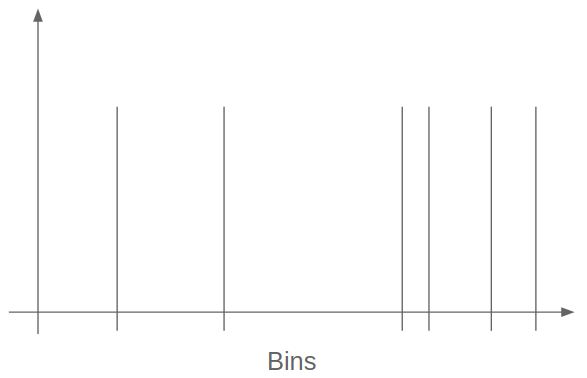
\includegraphics[scale=0.4]{figures/ref-bins.png}
      \caption[]{Reference equal-height histogram}
      \label{fig:ref-hist-bins}
    \end{center}
\end{figure}

Recall how an approximated histogram is built as explained in Section \ref{sec:ema-hist}. We will process each sample event by event and apply a discount factor per event, thus building an approximated histogram aggregation using the reference bins, for each feature of that sample. We compute multiple sample histograms to encode distributions over smaller time periods that may exist within the large reference period. We use an approximated histogram to mimic the target approximated histogram we will incrementally maintain in the streaming environment.

For each feature, we have now \textit{S} histograms, one for each sample. For each of the \textit{S} histograms we compute the distance between it and the reference histogram. Figure \ref{fig:compute-sample-distances} illustrates this process as we apply our distance function for each sample histogram and the reference histogram, obtaining \textit{S} distance measurements.

\begin{figure}[!htb]
    \begin{center}
      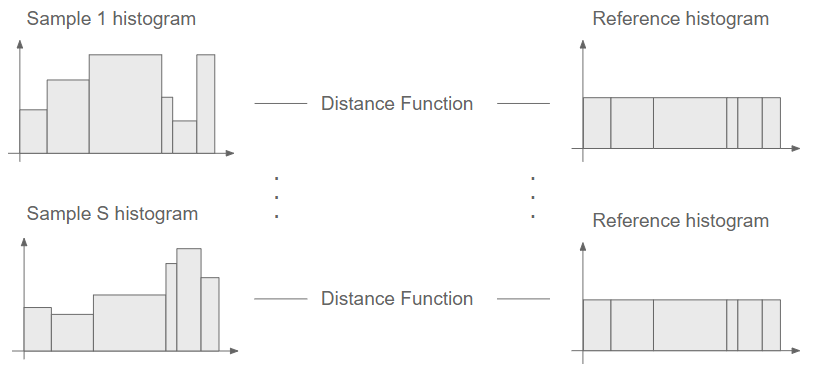
\includegraphics[scale=0.4]{figures/compute-sample-distances.png}
      \caption[Compute as many distance values as samples]{Compute as many distance values as samples, one for each sample-reference histogram pair}
      \label{fig:compute-sample-distances}
    \end{center}
\end{figure}

For each feature, we end up with \textit{S} distance values. These values are distance measurements between random samples of data and the reference period, and the histograms for each sample were built exactly like they will be maintained in streaming for better fidelity. Hence, we claim we now know the distribution of expected distance values. Given a new distance value measured between another window and the reference window, we can compute its probability and produce alerts if below a certain threshold.

\subsubsection*{Burn-in period at system initialization}
When we boot up our system in the streaming phase we initially have empty histogram aggregations. The period of time where you discard the alerts produced by the system until it processes enough data to produce accurate reports is commonly denoted as burn-in period. In order to avoid this burn-in period we propose that the sliding window approximate histogram aggregation for each feature is initialized using the last sample's histogram for that feature.

\subsubsection*{Batch phase artifacts}
For each feature, by the end of the batch phase, we have a reference histogram, a list of distance values that represents its distribution and the last sample's histogram to be used as burn-in period for the sliding window or target histogram.

\subsection{Streaming phase}

%- online phase:
          %  for each feature:
            %    1. initialize the streaming histogram as the last sample's histogram from the batch phase (burn-in period)
            
         %   for each event:
               % for each field/feature:
                  %  1. update the feature's streaming histogram (recall the update method)
                  %  2. compute the distance between the reference histogram and the target histogram
                   % 3. test the percentile the distance value fits according to the feature's distances list and alert if above a certain percentile (say the 99th)

           % introduce the multiple testing correction problem:
              %  "the more inferences are made, the more likely erroneous inferences are to occur"
             %   we are making multiple hypothesis testing when computing a distance and checking the percentile for each feature

                %introduce the Holm-Bonferroni multiple test correction method
            
            %So in reality we have:

          %  for each event:
               % for each field/feature:
                 %   1. update the feature's streaming histogram (recall the update method)
                  %  2. compute the distance between the reference histogram and the target histogram
                  %  3. apply holm-bonferroni for all feature's distances:
                     %   - each percentile will be a p-value
                    %    - order features by p-value
                    %    - check if p-value > FWER / (m + 1 - k)
                          %  if so then feature is divergent
                          
\subsection{Summary}